\chapter{Estado del arte}
\label{ch:chap02}

Este capítulo introduce un resumen de las áreas más importantes relacionadas al trabajo realizado en este proyecto, estas incluyen los modelos de iluminación por computadora, el método de radiosidad y sus posibles implementaciones y extensiones.

\section{Modelos de iluminación}
\label{sec:dibujado}

El proceso de dibujado de gráficos tridimiensionales por computadora comprende la generación automática de imágenes con cierto nivel de realismo a partir de modelos que componen una \textit{escena} o \textit{mundo} tridimencional, junto a un conjunto de cualidades físicas que rigen las formas en la que la luz interactúa con los objetos.

Trivialmente, esto puede ser reducido al problema de cálculo del valor de intensidad lumínica observada en un punto $x$ y proveniente de otro punto $x'$. En  \citeyear{Kajiya}, \citeauthor{Kajiya} presentó uno de los modelos más aceptado por la comunidad por su generalidad, comúnmente denominado <<la ecuación del \textit{rendering}>>:

\begin{equation}
    I(x,x') = g(x,x') \bigg[\epsilon(x,x') + \int_{S} \rho(x,x',x'')I(x',x'') \delta x''\bigg] \label{eq:rendering}
\end{equation}
donde:
\begin{itemize}
    \item $I(x,x')$ describe energía de radiación lumínica observada en el punto $x$ proveniente de $x''$
    \item $g(x,x')$ es un término geométrico, toma el valor de $0$ si existe oclusión entre $x'$ y $x$ en otro caso su valor es $\dfrac{1}{r^{2}}$ donde $r$ es la distancia entre $x'$ y $x$
    \item $\epsilon(x,x')$ mide la energía emitida por la superficie en el punto $x'$ a $x$
    \item $\int_{S} \rho(x,x',x'')I(x',x'') \delta x''$ está compuesta por dos términos:
        \begin{itemize}
            \item $\rho(x,x',x'')$ es el término de dispersión de la luz que llega desde $x''$ a $x$ desde el punto $x'$
            \item $I(x',x'')$ describe energía de radiación lumínica observada en el punto $x'$ proveniente de $x''$
        \end{itemize}
    por lo que este término refiere a la intensidad percibida desde $x$ considerando todos las reflexiones de
    luz posibles para el espacio $S$.
\end{itemize}

Existen distintos métodos de resolución de la <<ecuación del \textit{rendering}>>, la mayoría implican aproximaciones dado el gran costo de cálculo requerido para computar el valor exacto de $I(x,x')$. Estos métodos balancean el costo computacional de los algoritmos utilizados y la fidelidad con el valor final de la función. Dependiendo de las decisiones y simplificaciones consideradas existen dos clasificaciones posibles para el modelo: \textit{local} y \textit{global} \ref{local-vs-global-img}.

\vspace{5mm}
\begin{figure}[h]
	\begin{subfigure}{0.5\textwidth}
		  	\centering
   		 	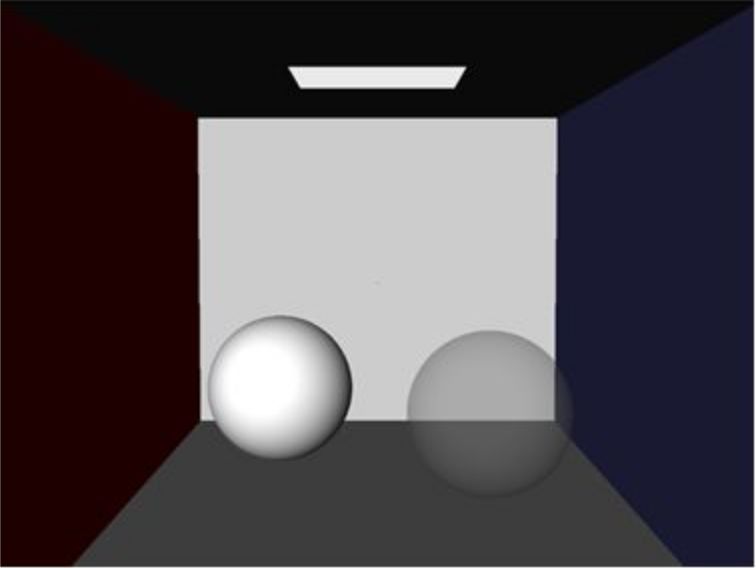
\includegraphics[width=1\linewidth]{assets/local}
   		 	\caption{Local}
   	\end{subfigure}
    \begin{subfigure}{0.5\textwidth}
    	\centering
    	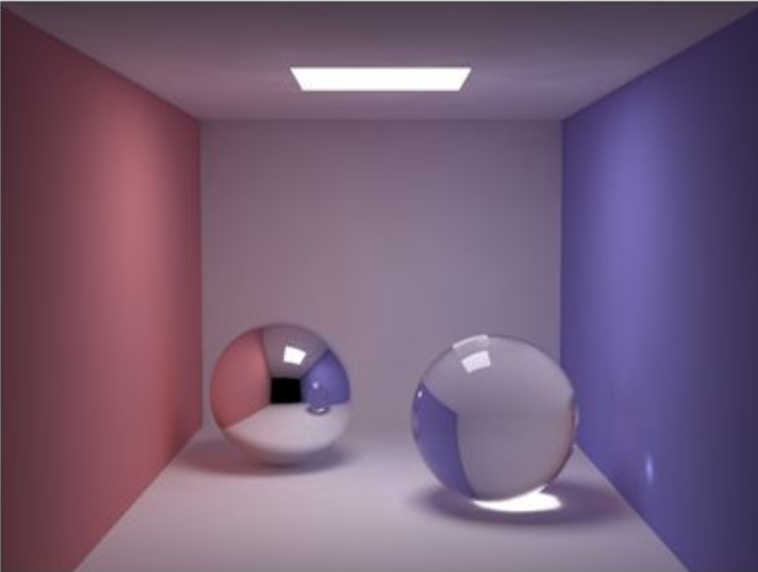
\includegraphics[width=1\linewidth]{assets/global}
    	\caption{Global}
    \end{subfigure}
    \caption{Dibujado utilizando distintos modelos de iluminación}
    \label{local-vs-global-img}
\end{figure}

\subsection{Iluminación Local}
\label{sec:ilumlocal}
Los modelos de iluminación local como el propuesto por \citeauthor{Phong} en \citeyear{Phong} tienen en cuenta las propiedades físicas de los materiales
y las superficies de forma individual. Es decir, al dibujar uno de los objetos no se toman en cuenta las posibles interacciones de los haces de luz con los objetos restantes en la escena. Estos métodos son frecuentemente utilizados en problemas cuya resolución debe ser realizada en tiempo real o por decisiones artísticas.

En referencia a la ecuación del rendering, el término geométrico nunca toma el valor 0 es decir, no se toma en cuenta las colisiones de la luz con otros objetos, $\epsilon(x,x')$ toma un valor constante únicamente dependiente de $x$ y $\int_{S} \rho(x,x',x'')I(x',x'') \delta x''$ toma el valor constante $1$.

\subsection{Iluminación Global}
\label{sec:ilumglobal}

El término iluminación global refiere a una modelo de computación gráfica en donde se simulan parcialmente o completamente las interacciones de la luz con todos los objetos que se encuentran  en la escena. Es decir, en contraposición a la iluminación local, se consideran los fenómenos de reflexión y refracción de la luz.

Dependiendo de las característica de los modelos y algoritmos empleados, pueden obtenerse resultados más fieles a la realidad en distintos sentidos.

El algoritmo de \textit{trazado de caminos de rayos} emula completamente cada haz de luz desde su incepción en una fuente luminosa siguiendo el camino de interacciones del rayo con las distintas superficies de la escena. En este caso el grado de granularidad (que depende directamente de la cantidad de muestras utilizadas) impacta directamente en los errores y calidad en la imagen final.

Por otro lado, el algoritmo de \textit{mapeado de fotones} simula los efectos producidos por las colisiones de las partículas que componen la luz (fotones) con los objetos, que dejan \textit{impresiones} que afectarán el resultado final de la imágen.

Existen además distintas variaciones e híbridos de estos métodos que normalmente dibujan imágenes \textit{fuera de línea} pues son demasiado costosos como para dibujar imágenes en tiempo real.

\section{Radiosidad}
\label{sec:radiosidad}

El método de radiosidad es una técnica de iluminación global \ref{sec:ilumglobal} que emula el transporte de la luz entre superficies que se rige por la magnitud física definida, a su vez, como radiosidad, que indica el flujo de energía irradiada por unidad de área ($\frac{W}{m^{2}}$).

Originalmente, este modelo de iluminación global fue propuesto por \citeauthor{Goral} en \citeyear{Goral}, se basa en modelos matemáticos similares a los que resuelven el problema de la transferencia de calor en sistemas cerrados (MEF).

\subsection{Radiosidad en superficies lambertianas}

La solución propuesta por \citeauthor{Goral} implica que todas las superficies son idealmente difusas, también conocidas como \textbf{lambertianas}. Estas superficies se comportan como reflectores difusos ideales, lo que significa que reflejan la energía incidente de forma isotrópica siguiendo la regla del coseno como se observa en la figura \ref{img:lamber}.

\vspace{5mm}
\begin{figure}[h]
	\centering
	\begin{subfigure}{0.45\textwidth}
		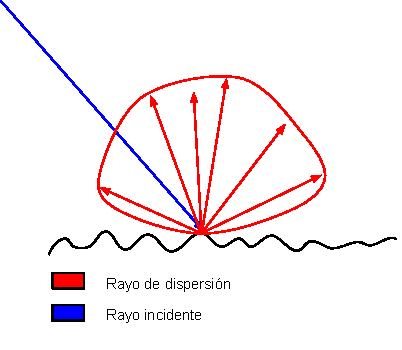
\includegraphics[width=1\linewidth]{assets/difusa}
		\caption{Reflector genérico}
	\end{subfigure}
	\begin{subfigure}{0.45\textwidth}
		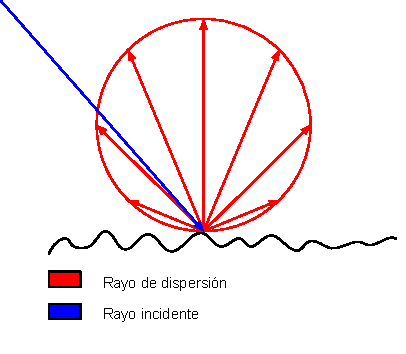
\includegraphics[width=1\linewidth]{assets/lambert}
		\caption{Reflector lambertiano}
	\end{subfigure}
	\caption{Comparación entre tipos de reflectores}
	\label{img:lamber}
\end{figure}

Adicionalmente, se considerará que cada superficie irradia energía lumínica en todas direcciones en un diferencial de área $\delta_{A}$, para una dirección de vista $\omega$ puede ser definida como:

\begin{equation}
    i = \frac{\delta{P}}{\cos{\phi\delta\omega}} \label{eq:i}
\end{equation}
donde:
\begin{itemize}
    \item $i$ es la intensidad de la radiación para un punto de vista particular
    \item $\delta{P}$ es lae energía de la radiación que hemana la superficie en al dirección $\phi$ con ángulo sólido $\delta\omega$
\end{itemize}

En superficies perfectamente lambertianas, la energía reflejada puede ser expresada como: $\frac{\delta{P}}{\delta{\omega}} = k\cos{\phi}$. Donde $k$ es una constante.
Sustituyendo en \eqref{eq:i} se obtiene: $\frac{\delta{P}}{\delta{\omega}} = \frac{k\cos{\phi}}{\cos{\phi}} = k$, esto implica que la energía percibida de un punto $x$ 
es constante, independientemente del punto de vista.

Es por esto que la energía total que deja una superficie ($P$) puede ser calculada integrando la energía que deja la superficie en cada dirección posible, esto es, se integra la energía saliente en un hemi-esfera centrada en el punto estudiado:

\begin{equation}
    P = \int_{2\pi} \delta{P} = \int_{2\pi} i\cos{\phi}\delta{\omega} = i \int_{2\pi} \cos{\phi}\delta{\omega} = i\pi
    \label{eq:P}
\end{equation}

Por tanto, dada una superficie $S_{i}$, es posible calcular la energía lumínica que deja la superficie utilizando \eqref{eq:P}.

Existen tres métodos posibles de cálculo de la ecuación de radiosidad: la integración basada en elementos finitos, la integración basada en reglas de cuadratura y la integración basada en métodos de Monte Carlo.

En este caso, los autores decidieron utilizar el método de elementos finitos, para poder aplicarlo resta definir la \textit{cerradura} de una superficie, definiremos la cerradura de una superficie como los límites que definen los puntos internos y externos de esta, llamaremos \textit{parche} a cada una de estas superficies cerradas. Esto hace que el problema sea resoluble utilizando métodos de elementos finitos, con esta re-formulación del problema, es fácilmente trasladable a la ecuación \eqref{eq:rendering}.

\begin{equation}
    B_{j} = E_{j} + \rho_{j} \sum_{i=1}{N} B_{i} F_{ij} \label{eq:radiosity}
\end{equation}
donde:
\begin{itemize}
    \item $B_{j}$ es la intensidad lumínica (radiosidad) que deja la superficie $j$.
    \item $E_{j}$ es la intensidad lumínica directamente emitida por $j$.
    \item $\rho_{j}$ es la reflectividad del material para la superficie $j$.
    \item $F_{ij}$ se denomina \textit{factor de forma}, un término que representa la fracción de energía lumínica
    que deja la superficie $i$ y llega a $j$. 
\end{itemize}

Cabe destacar que la naturaleza recursiva de la ecuación anterior, implica que se toman en cuenta todas las reflexiones difusas que existan en la escena. Como puede observarse, resolver el sistema de $N$ ecuaciones lineales bastaría para conocer la energía emitida por cada parche. 

$E$, $\mathbf{\rho}$ dependen de los materiales que compongan la escena, son parámetros dados. Sin embargo, resta computar la matriz de factores de forma $\mathbf{F}$ para finalmente obtener el vector de radiosidades $B$. 

Para determinar una entrada de la matriz $F_{ij}$ involucrando a las superficies $i$ y $j$ de área $A(i)$, $A(j)$, considerando los diferenciales infinitesimales de área $\delta{A_{i}}$, $\delta{A_{j}}$, representados en la figura \ref{img:ff}, el ángulo sólido visto por $\delta{A_{i}}$ es $\delta{\omega} = \frac{\cos{\phi_{j}\delta{A_{j}}}}{r^{2}}$. Sustituyendo en \eqref{eq:P} se obtiene:

\begin{equation}
    \delta{P}_{i}\delta{A_{i}} = i_{i} \cos{\phi_{i}}\delta{\omega}\delta{A_{i}} = \frac{P_{i}\cos{\phi_{i}}\cos{\phi_{j}}\delta{A_{i}}\delta{A_{j}}}{\pi r^{2}}
\end{equation}

\vspace{5mm}
\begin{figure}[h]
	\centering
	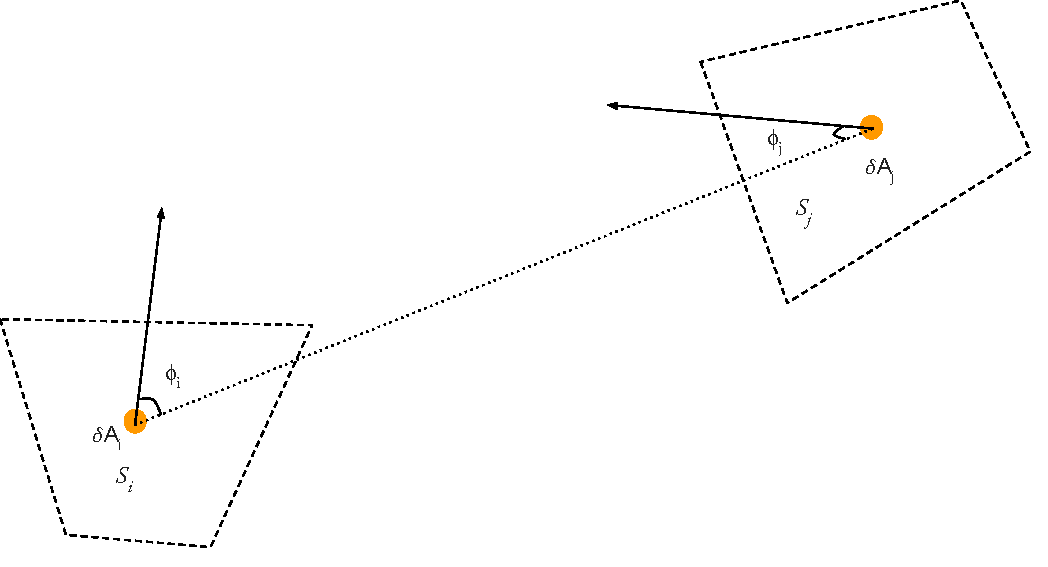
\includegraphics[width=0.8\linewidth]{assets/ff}
	\captionof{figure}{El factor de forma entre dos superficies}
	\label{img:ff}
\end{figure}


Considerando que ${P}_{i}{A_{i}}$ es la energía que deja $i$, y que el factor de forma $F_{ij}$ representa el porcentaje de dicha energía que llega a $j$ podemos observar que:

\begin{equation}
    F_{\delta{A_{i}}-\delta{A_{j}}} = \frac{\frac{P_{i}\cos{\phi_{i}}\cos{\phi_{j}}\delta{A_{i}}\delta{A_{j}}}{\pi r^{2}}}{P_{i}\delta{A_{i}}} = \frac{\cos{\phi_{i}}\cos{\phi_{j}}\delta{A_{i}}}{\pi{r^{2}}}
\end{equation}

Integrando, para obtener el factor de forma para el área total:

\begin{equation}
    F_{ij} = \frac{1}{A_{i}} \int_{A_{i}}\int_{A_{j}}\frac{\cos{\phi_{i}}\cos{\phi_{j}}\delta{A_{i}}\delta{A_{j}}}{\pi{r^{2}}} \label{eq:ff}    
\end{equation}

De \eqref{eq:ff} se obtienen las siguientes propiedades:
\begin{enumerate}
	\label{propsff}
    \item $A_{i}F_{ij} = A_{j}F{ji}$
    \item $\sum_{j=1}^{N} F_{ij} = 1$
    \item $F_{ii} = 0$
    \item $F_{ij}$ toma el valor correspondiente a la proyección de $j$ en una hemiesfera unitaria centrada en $i$, proyectándola a su vez en un disco unitario.
\end{enumerate}


\section{Métodos de cálculo de la matriz de Factores de Forma}
\label{sec:calculoff}

El cálculo de los factores de forma a través de la ecuación \eqref{eq:ff} analíticamente es inviable en la práctica pues supone la necesidad de calcular la visibilidad entre cada par de parches que componen la escana. Por tanto, es necesario establecer otros métodos que provean aproximaciones lo suficientemente correctas.

Geométricamente, puese establecerse una analogía para la computación de factores de forma conocida como <<analogía de Nussel>>. Se expresará el factor de forma como la proporción de área proyectada de $S_{j}$ en una hemi-esfera centrada en $S_{i}$ y luego en un disco centrado en $S_{i}$.

El cálculo de la matriz de factores de forma $\mathbf{F}$ supone la proyección de los parches, de aquí en más se asumirá que estos parches son poligonales y por tanto es posible utilizar las técnicas de dibujado de objetos tridimensionales tradicionales.

\subsection{Rasterización}

El <<\textit{rendering pipeline}>> es un proceso de dibujado estandarizado que consiste en un conjunto de etapas cuyo cometido es la generación de un \textit{frame buffer}. Los fabricantes de los dispositivos aceleradores gráficos y/o sistemas operativos proveen de interfaces de programación (OpenGL, Vulkan, DirectX) que se basan en este modelo para abstraer el uso del hardware.

Si bien el <<\textit{rendering pipeline}>> es modificable, cada una de sus etapas están definidas.  El programador es capaz de modificar pequeñas funciones (también llamadas \textit{kernels} o \textit{shaders}) que son ejecutadas en la GPU en las etapas correspondientes. El cometido de estas funciones es la transformación los parámetros de entrada en parámetros que recibirá la siguiente etapa. A continuación, se describe el proceso para OpenGL 4.5 \ref{img:pipelinegl} visualizado en la figura \ref{img:pipelinegl}, aunque muchas de estas etapas son trasladables a otras tecnologías existentes.

\vspace{5mm}
\begin{figure}[H]
	\centering
	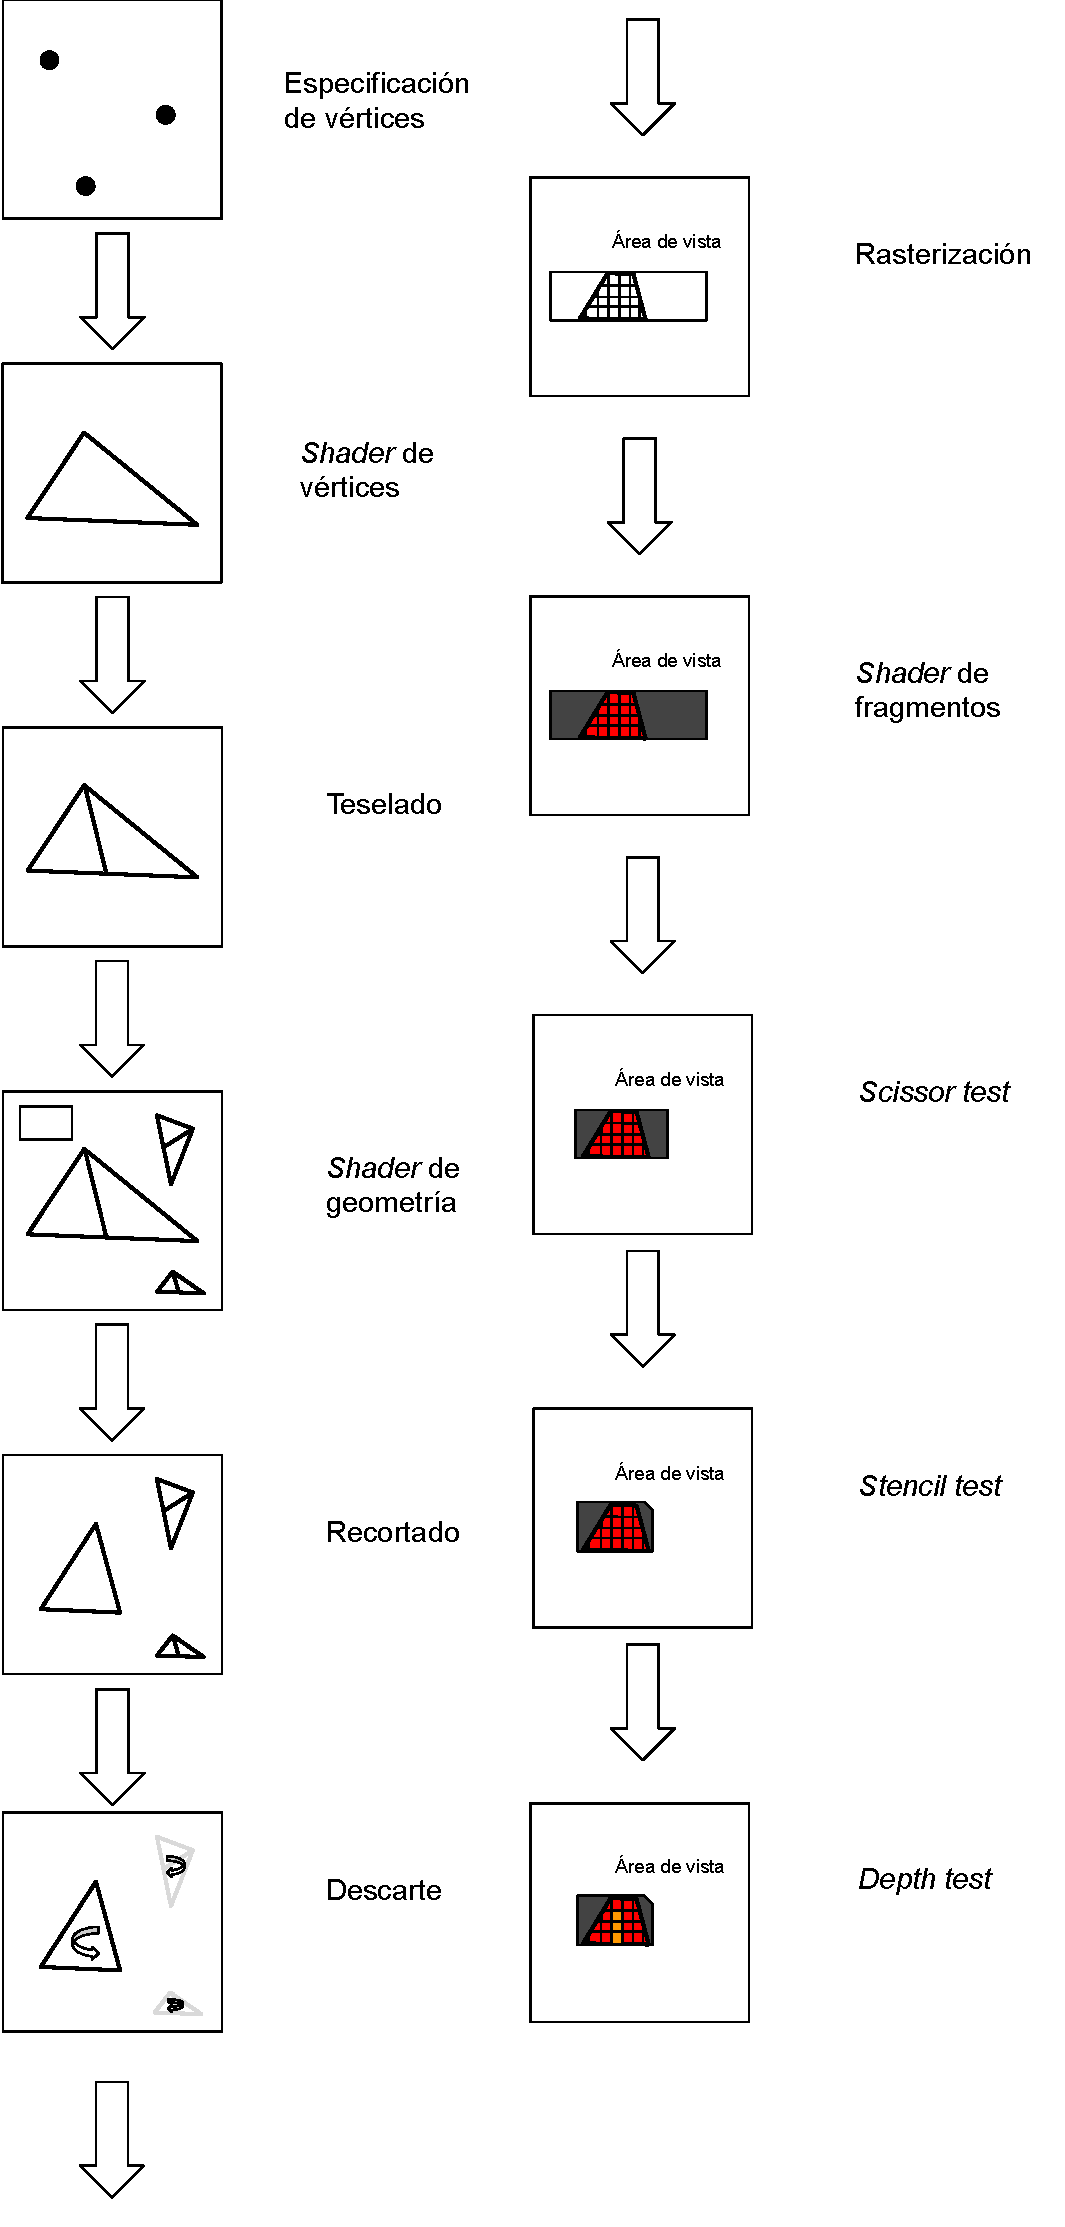
\includegraphics[width=0.55\linewidth]{assets/OpenGL}
	\captionof{figure}{El \textit{rendering pipeline} de OpenGL}
	\label{img:pipelinegl}
\end{figure}
\begin{enumerate}
	\item Procesamiento de primitivas geométricas:
		\begin{enumerate}
			\item Especificación de vértices: Inicialmente, las aplicaciones indican un conjunto de vértices a dibujar, definiendo cierto conjunto de primitivas geométricas como triángulos, cuadriláteros, puntos, líneas u otros.
			\item \textit{Vertex shader}: Esta etapa transforma los vértices de entrada suministrados por la aplicación. Generalmente se computan las transformaciones lineales necesarias para cambiar la base de las coordenadas de los vértices de un sistema local al sistema global que defina la aplicación. Las coordenadas retornadas deberán corresponderse con coordenadas del espacio de recorte. Es decir, coordenadas correspondientes al volumen de vista.
			\item Teselado: En esta etapa se procesan los vértices a nivel de primitiva geométrica, con el objetivo de subdividirlas para mejorar la resolución obtenida.
			\item \textit{Geometry shader}: En esta etapa también se procesan los vértices a nivel de primitiva geométrica con el objetivo de mutarlas y replicarlas.
			\item Recortado: Esta etapa es \textit{fija}, es decir, no es programable. Todas las primitivas calculadas anteriormente que residan fuera del volumen de vista serán descartadas en las etapas futuras. Además, se transforma las primitivas a coordenadas de espacio de ventana.
			\item Descarte: El proceso de descarte (en inglés \textit{culling}), es también fijo. Consiste en la eliminación de primitivas que no cumplan ciertas condiciones, como por ejemplo el descarte de caras cuya normal tiene dirección opuesta a la del observador.
		\end{enumerate}
	\item Procesamiento de fragmentos (rasterización):
		\begin{enumerate}
			\item Rasterización: El proceso de rasterización discretiza las pirmitivas en espacio de pantalla en un conjunto de fragmentos.
			\item \textit{Shader de fragmentos}: El procesamiento de cada fragmento se realiza a través del \textit{shader de fragmentos} que calcula uno o más colores, un valor de profundidad, y valores de plantilla (del inglés \textit{stencil}).
			\item \textit{Scissor test}: Todos los fragmentos fuera de un área rectangular definida por la aplicación son descartados.
			\item \textit{Stencil test}: Los fragmentos que no pasan la función de planilla definida por la aplicación no son dibujados, por ejemplo, simular el \textit{scissor test} que requieran primitivas más complejas.
			\item \textit{Depth test}: En esta etapa se ejecuta el algoritmo del Z-Buffer, donde sólo se escribirá el resultado en el \textit{frame buffer} de aquellos fragmentos que tengan la menor profundidad. Es decir, los que se encuentren más cerca del observador.
		\end{enumerate}
\end{enumerate}

Esta técnica de dibujado es extremadamente rápida, además, la mayoría de dispositivos contienen hardware especializado capaz de acelerar estos cálculos, comúnmente conocidos como Unidades de Procesamiento Gráfico (o GPU en sus siglas en inglés). Con el objetivo de aprovechar este hardware \citeauthor{Cohen} idearon el método del hemi-cubo para el cálculo de factores de forma.

\subsubsection{El método del hemi-cubo}

El hardware optimizado para realizar operaciones de rasterización tiene la capacidad de proyectar escenas tridimensionales en imágenes bidimencionales a gran velocidad.

Para utilizar el hardware eficientemente consideraremos que se calculará una fila completa de $\mathbf{F}$, esto implica que dada $S_{i}$, una superficie, calcularemos simultáneamente los factores de forma para las superficies restantes. 

El método original propone la proyección de la escena una hemiesfera centrada en $S_{i}$, sin embargo los modelos de proyección utilizados no lo permiten. Por esto es necesario proyectar la escena a un hemi-cubo centrado en $S_{i}$, esto supone el dibujado de cinco superficies bidimensionales, y por tanto puede ser realizada utilizando la rasterización.

Este método aprovecha el buffer de profundidad (Z-buffer), tomando en cuenta los píxeles proyectados para los elementos que se encuentren más cercanos al parche $S_{i}$.

El algoritmo, propuesto originalmente por \citeauthor{Cohen} en \citeyear{Cohen}, propone rasterizar la escena tridimencional en cinco texturas correspondientes al hemicubo, para cada pixel renderizado se sumará un valor diferencial del factor de forma, que dependerá de la posición del píxel en el hemi-cubo en relación a la hemiesfera que este aproxima. Esta suma genera una fila de la matriz $\mathbf{F}$, específicamente la fila $\mathbf{F}_{i}$.

Por tanto, podremos definir:

\begin{equation}
	\mathbf{F}_{ij} = \sum_{q=1}^{R} \delta{F_{q}}
	\label{eq:ffgreenberg}
\end{equation}
donde:
\begin{itemize}
	\item $R$ es la cantidad de píxeles correspondientes a la superficie $S_{j}$ que cubren el hemi-cubo.
	\item $\delta{F_{q}}$ el diferencial de factor de forma asociado al píxel del hemi-cubo $q$.
\end{itemize}

\vspace{5mm}
\begin{figure}[H]
	\centering
	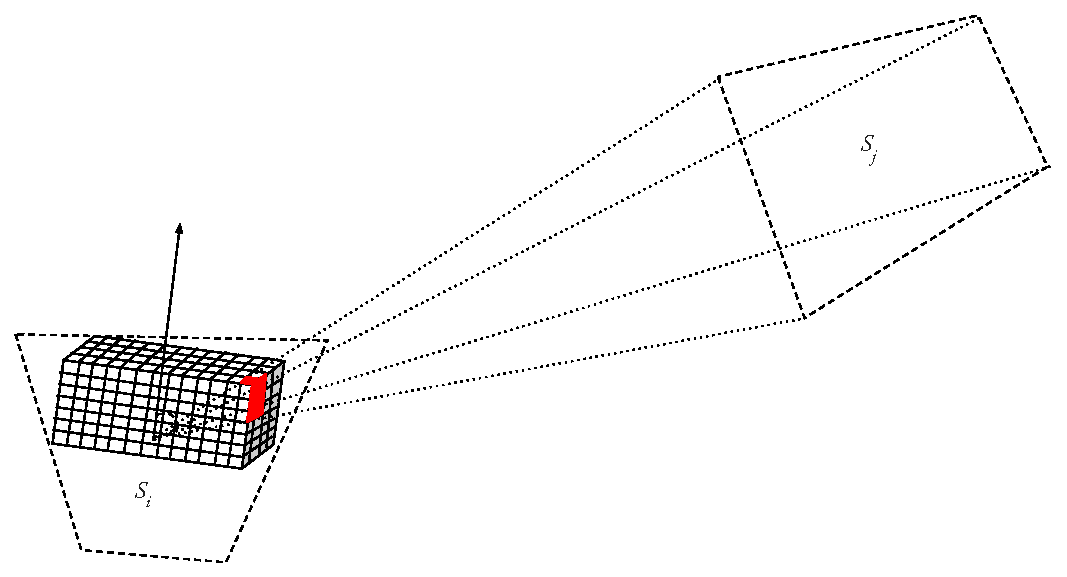
\includegraphics[width=0.8\linewidth]{assets/Hemicube}
	\captionof{figure}{Representación gráfica del método del hemicubo}
	\label{img:ff}
\end{figure}

Los diferenciales de factores de forma deben corregir la deformación introducida con el cambio de proyección desde una hemiesfera a un hemi-cubo, para ello, para cada píxel que compone el hemi-cubo es necesario calcular la proporición de área que este término ocupa en la hemiesfera unitaria.

Para la cara superior, los diferenciales se calculan como:

\begin{equation}
	\delta{F_{q}} = \frac{\cos{\phi_{i}}\cos{\phi_{j}}}{\pi{r^{2}}} \delta{A} = \frac{\delta{A}}{\pi({x^{2} + y^{2} + 1})} 
\end{equation}

Para las caras laterales, la fórmula dada es:

\begin{equation}
\delta{F_{q}} = \frac{\cos{\phi_{i}}\cos{\phi_{j}}}{\pi{r^{2}}}\delta{A} = \frac{z\delta{A}}{\pi({x^{2} + z^{2} + 1})}
\end{equation}


\subsection{Trazado de rayos}
\label{sec:raytracing}

Otra de las técnicas de emulación de iluminación existente es el trazado de rayos, consiste en la computación de los puntos de intersección de una semi-recta (a la que denominaremos rayo) con la geometría de la escena, cada uno de estos rayos emulará el transporte de los haces de luz emitidos.

Para cada uno de los rayos emitidos, se determinará el punto de intersección más cercano, luego es posible establecer qué primitiva geométrica fue interceptada es posible integrar el resultado intermedio producido por la intersección al resultado final, dependiendo del modelo de iluminación utilizado.

El trazado de rayos es una técnica efectiva \cite{Kajiya} para computar la ecuación del rendering, utilizando la técnica de \textit{trazado de camino} donde el haz de luz absorbe las propiedades de los materiales con los que interacciona. En este algoritmo, cada uno de los rayos emitidos computa uno de los integrandos de la ecuación.

\subsubsection{El método de la hemi-esfera}

En el caso de la radiosidad, es posible utilizar esta técnica para calcular los factores de forma, es decir, para resolver la ecuación \eqref{eq:ff}.

Recordando, un factor de forma $\mathbf{F}_{ij}$ representa la energía que llega a la superficie $S_{i}$ desde $S_{j}$, es posible re-imaginar el problema original colocando una hemi-esfera unitaria en el centro de $S_{i}$ orientada en la direccción de la normal de la superficie.

El algoritmo propuesto por \citeauthor{Malley}  consiste realizar un muestreo de la cantidad de  rayos que parten desde el centro de $S_{i}$ e intersecan $S_{j}$, las direcciones de los rayos serán determinadas a partir de la \textit{distribución del coseno} cuya función de densidad es $f(x) = \frac{1}{2}[1 + \cos((x-1)\pi)]$.

\begin{equation}
	\mathbf{F}_{ij} = \sum_{k=1}^{nMuestras} \frac{\beta(ray(S_{i},d), S_{j})}{nMuestras} \text{ donde } d \text{ tiene una distribución apropiada}.
	\label{eq:ffhemiesfera}
\end{equation}
donde:

$\beta(r, S_{x})$ toma el valor $1$ si el rayo $ray(S_{i},d)$ interseca a $S_{j}$ o $0$ en otro caso.

\vspace{5mm}
\begin{figure}[H]
	\centering
	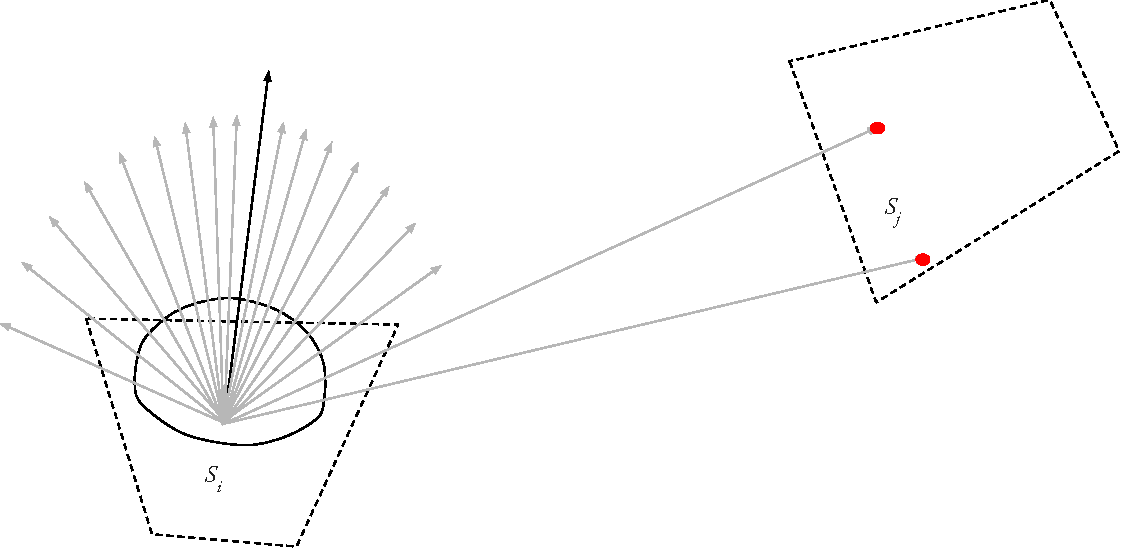
\includegraphics[width=\linewidth]{assets/Raytracing}
	\captionof{figure}{Representación gráfica del método de método de trazado de rayos}
	\label{img:ff}
\end{figure}

\section{Superficies especulares}

Originalmente, el método de cálculo de la radiosidad asume que todas las superficies son reflectores lambertianos, lo que supone que solo existirán reflexiones difusas cuando la luz interactúa con ellas. Sin embargo, es necesario simular reflexiones especulares correctamente para obtener resultados que se asemejen a la realidad.

Por ello existe la extensión del método para superficies especulares o refractantes propuesto por \citeauthor{Sillion} en \citeyear{Sillion}. Los autores proponen extender el significado del término \textit{factor de forma} a más que una mera relación geométrica entre parches. Sino que un factor de forma $\mathbf{F}_{ij}$ será la proporción de energía que deja la superficie $i$ y llega la superficie $j$ luego de un número de reflexiones y refracciones.

Esto modifica completamente los algoritmos de cálculo de factores de forma, loa autores proponen un algoritmo de  que cálculo consiste en el trazado de rayos desde $S_{i}$ en una dirección arbitraria $d$ bien distribuida.  Luego, una vez que se conozca el \textbf{camino} trazado se distribuirá el valor final del factor de forma dependiendo en la cantidad de superficies con las que interaccione el rayo y sus coeficientes especulares como se observa en la figura \ref{img:caminoespecular}.

\vspace{5mm}
\begin{figure}[H]
	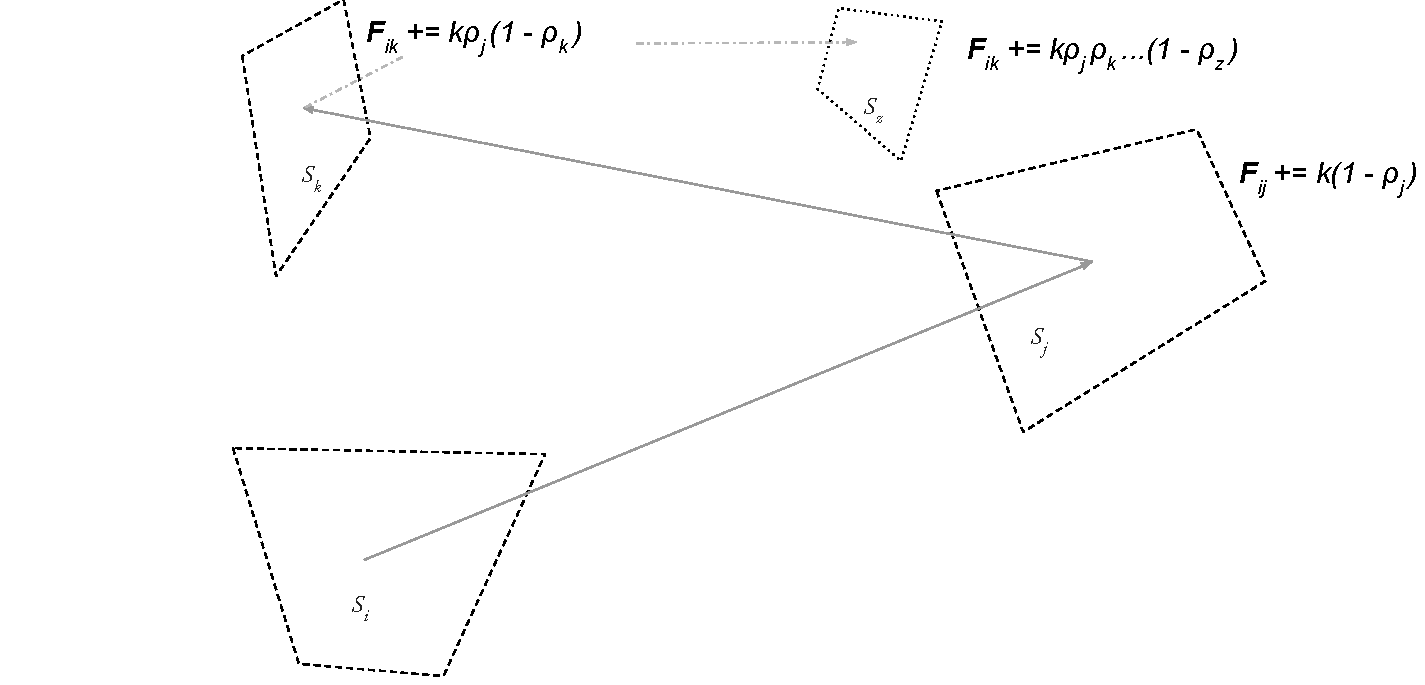
\includegraphics[width=1\linewidth]{assets/extended}
	\captionof{figure}{Representación gráfica del cálculo del factor de forma extendido donde $k$ corresponde al inverso de la cantidad de muestras tomadas.}
	\label{img:caminoespecular}
\end{figure}

\section{Cálculo del vector de radiosidades}

Luego de computar la matriz $\mathbf{F}$ y dado los vectores de emisiones $E$ y reflexiones $\rho$, resta computar el vector de radiosidades correspondiente para cada parche, denominado $B$.

Recordando \eqref{eq:radiosity}, es posible deducir el problema al sistema de ecuaciones dado por:

\begin{equation}
	E = (\mathbf{I} - \mathbf{RF})B
\end{equation}

Los estudios de álgebra lineal modernos permiten la resolución de sistemas de ecuaciones de forma optimizada, dependiendo de las propiedades observadas.

Recordando las propiedades en \ref{propsff}, podemos observar que:

\begin{itemize}
	\item $\sum_{j=1}^{N} \mathbf{F}_{ij} \leq 1 \forall{i \in [1,N]}$
	\item $\rho_{i} \leq 1 \rightarrow \sum_{j=1}^{N} \mathbf{R}_{ij} \leq 1 \forall{i \in [1,N]}$
\end{itemize}

Esto implica que las entradas de $\mathbf{RF}$ s\texttt{}on siempre menores a $1$, por tanto, $(\mathbf{I} - \mathbf{RF}) = M$ es diagonal dominante ya que $\sum_{j=1}^{N}|R_{ij}F_{ij}| \le 1 \forall i \in [1, N]$ y $R_{ii}F_{ii} = 0  \forall  i \in [1,N]$. Esto garantiza la convergencia del uso de métodos de resolución iterativos, como el algoritmo de Gauss-Seidel.

Si bien existen maneras alternativas de resolución del sistema planteado con consideraciones específicas del problema, a efectos de esta investigación se considerarán los métodos de resolución de ecuaciones lineales que requieran a lo sumo esta propiedad.

Cabe aclarar, que el método planteado hasta el momento resuelve la radiosidad en un único canal. Es decir, no se toma en cuenta todo el espectro electromagnético de la luz, es por ello que puede establecerse una extensión del método. Esta extensión implica la existencia de tres vectores de reflexión, uno para cada canal \textit{RGB} (del inglés \textit{Red - Green - Blue}. Por tanto es necesario que se resuelvan tres y no un único sistema de ecuaciones, aunque es posible destacar que la matriz $\mathbf{F}$ permanece constante pues depende únicamente del coeficiente de reflexión especular y la geometría de la escena, el único cambio en el sistema surge en la matriz $\mathbf{R}$ que pasará a depender del canal seleccionado: $\mathbf{R}_{c}$.